\documentclass{ximera}

\title{Deploying Ximera documents}
\author{Bart Snapp}

\begin{document}
\pdfOnly{\onecolumn}
\begin{abstract}
    Deploying Ximera documents.
\end{abstract}
\maketitle
\pdfOnly{\begin{multicols}{2}}
        We have several options for deploying Ximera documents: Deploying through a
        GitHub codespace, deploying from your machine, and deploying though a GitHub
        action. We will discuss the first option here and suggest the interested user
        reach out to Ximera developers for help with other deploy methods. With all
        options you will need a
        \verb!GPG_KEY_ID! and a \verb!GPG_KEY!. These will identify your ``xourse name'' as one that you own.
        
        \section{Obtaining GPG Keys}

        If you are deploying legacy Ximera material, you may need to contact Ximera
        developers to obtain a proper key. If you are deploying new Ximera content,
        you can get your own GPG key by pressing ``SERVE'' in a \textit{fresh} codespace. If
        you do this, and you want to ``officially'' deploy, you should tell us your
        name and email address:
        \pdfOnly{\end{multicols}}\pdfOnly{\enlargethispage{2em}}
\begin{image}
    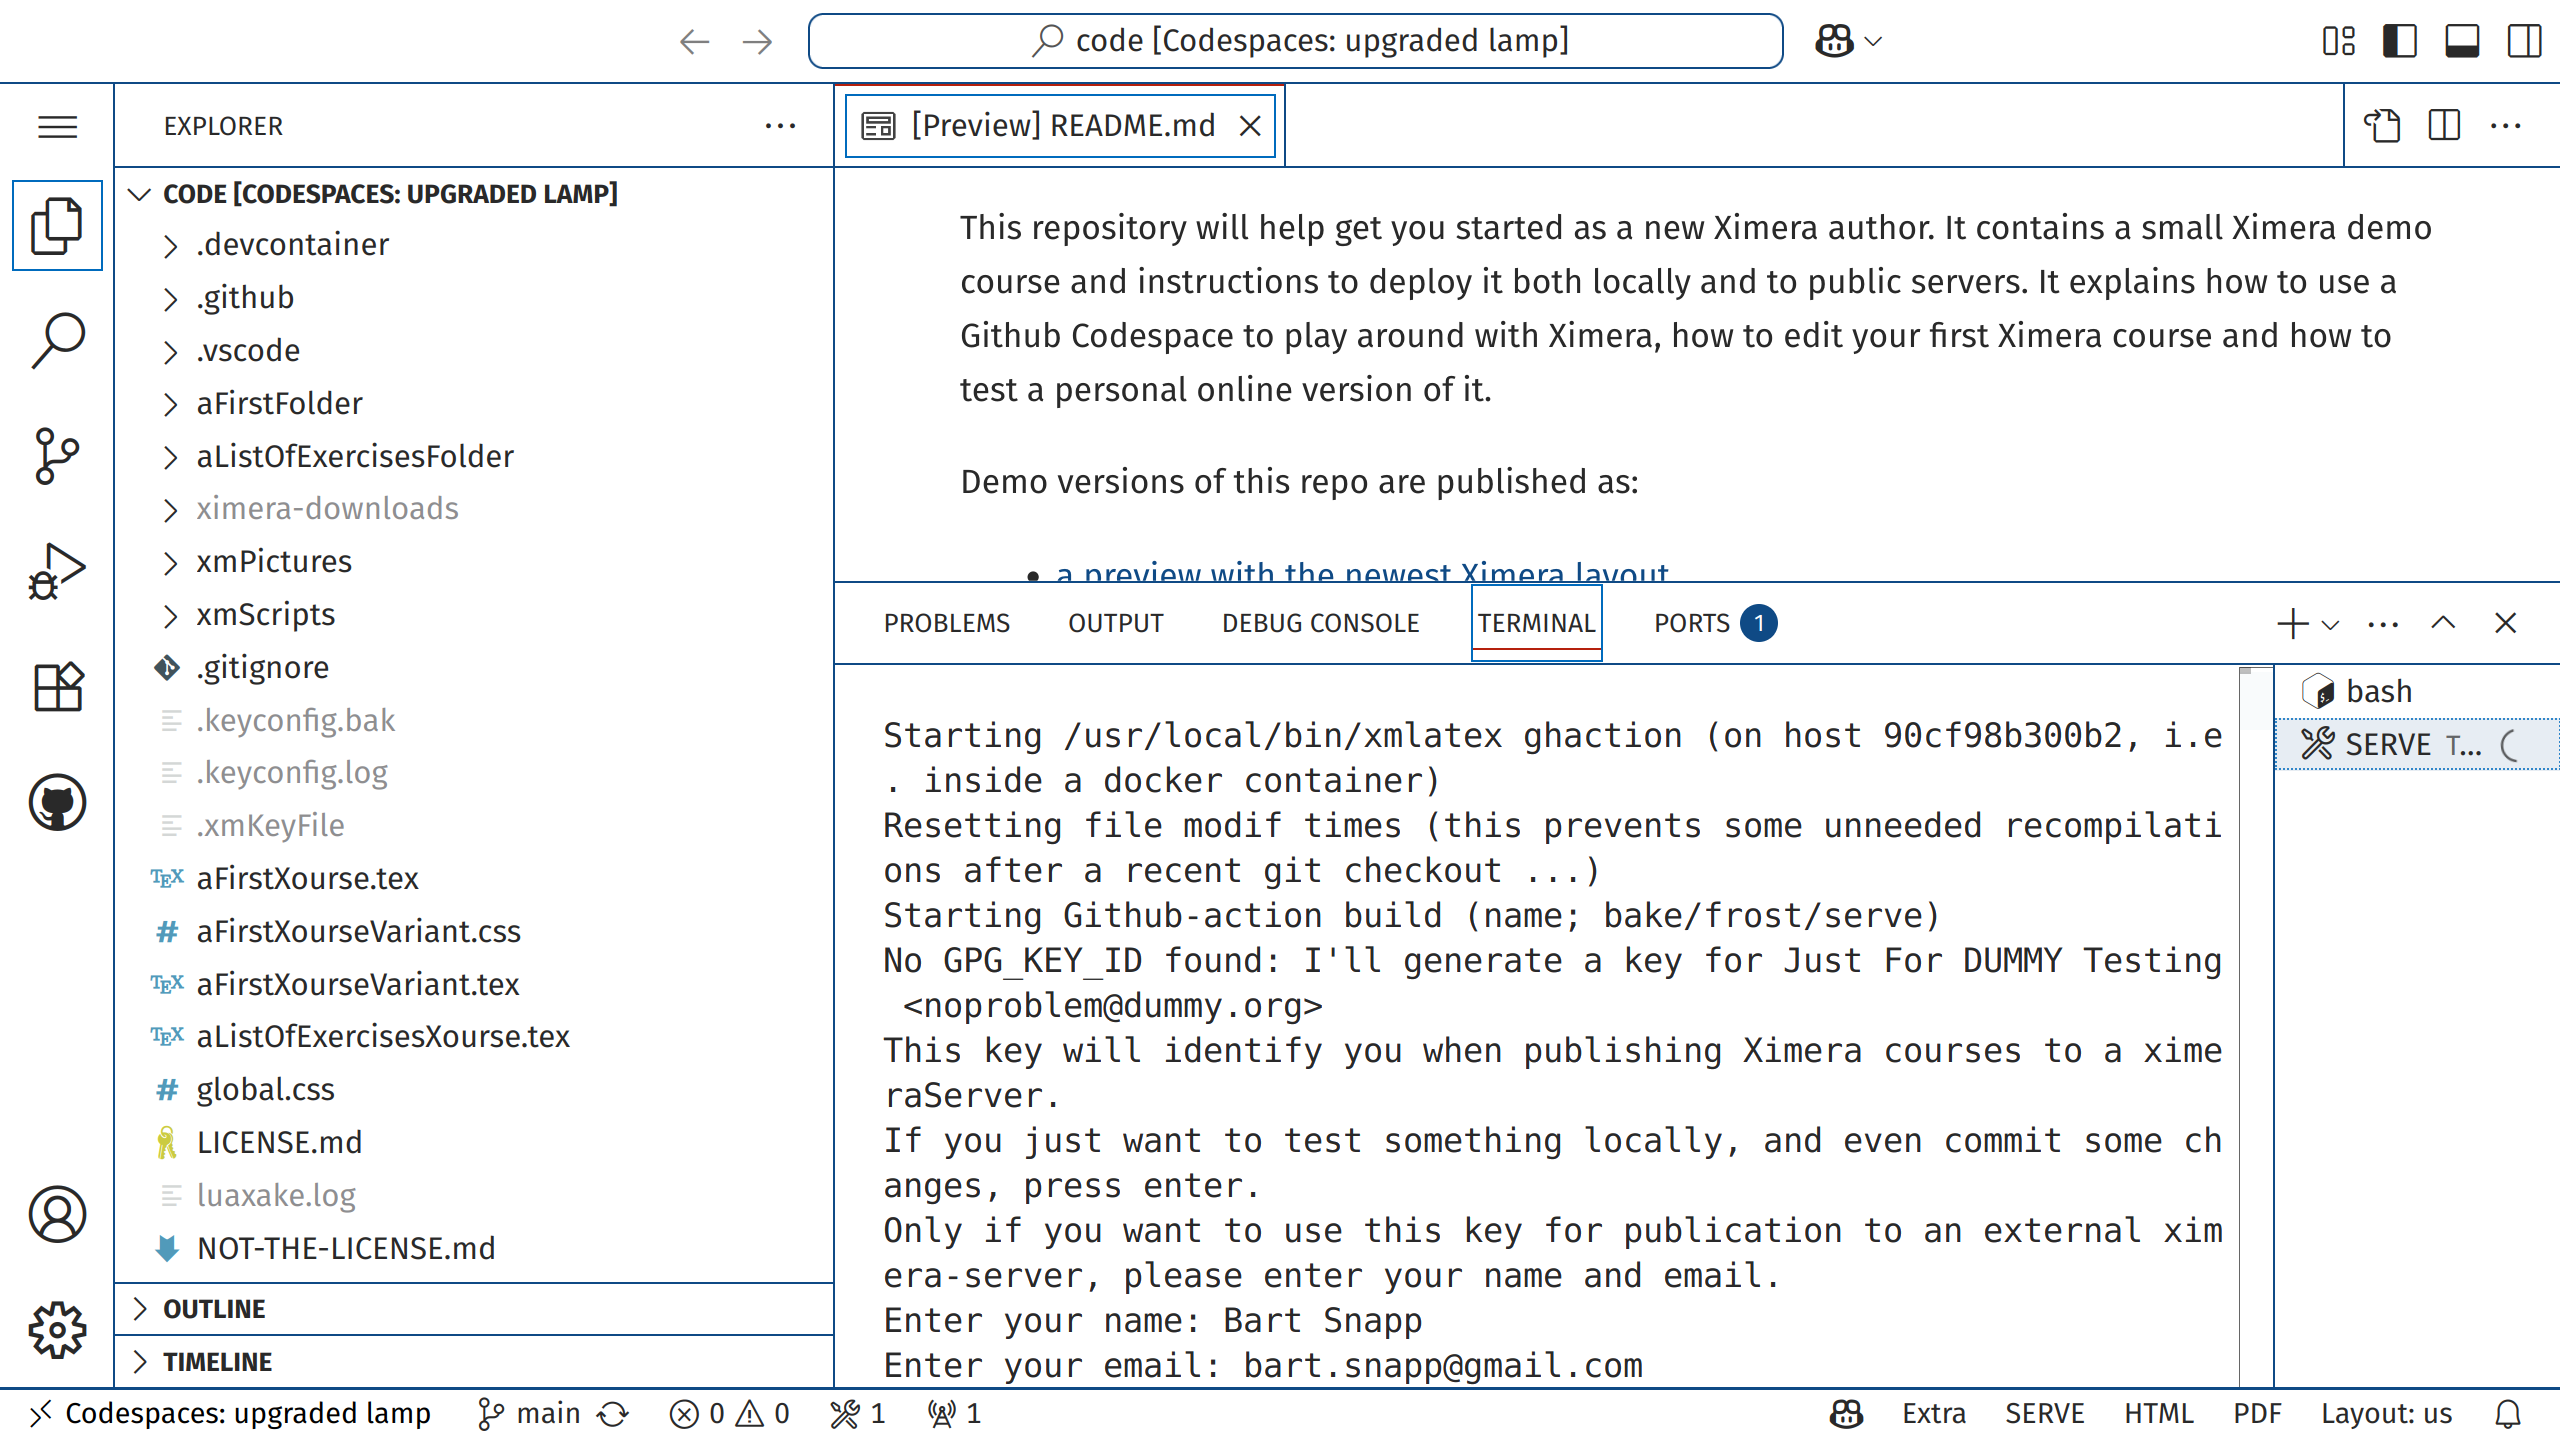
\includegraphics[width=.7\textwidth]{xfsEmail}
\end{image}
\pdfOnly{\newpage}
\pdfOnly{\begin{multicols*}{2}}
    
        Open the file (using `hamburger' $\to$ File $\to$ open-file) \verb!.xmKeyFile!.
        It should look something like this:
        {\pdfOnly{\footnotesize}\begin{verbatim}
# This file contains a private GPG key for 
# Bart Snapp <bart.snapp@gmail.com> 
# to publish Ximera courses.
#
# These settings will be overwritten by existing 
# GitHub environment variables
#
# GPG_KEY_ID and GPG_KEY
#
#   *** DO NOT COMMIT THIS FILE ***
#
GPG_KEY_ID=215FC33FAB44D5CCA31A04B2CC78CB561FDC49A8
GPG_KEY="\
LS0tLS1CRUdJTiBQR1AgUFJJVkFURSBLRVkgQkxPQ0stLS0tLQoKbEZnRVp2QUFBaFlKS3dZQkJB
SGFSdzhCQVFkQUI4UW9zbWR3YmJBcHJHQ1k1N3Q1VmRVVkJGTlpWWEFQTGVkWQpMWnZtQ0tjQUFR
QzF4dmlVckwzRWE2bmpJcUZ1WitWL2EzUG55TCtPeDMvTHg3eWxtV2pNNlJUeHRDTkVkVzF0CmVT
QkdiM0lnV0dsdFpYSmhJRHh1YjI1bFFHVjRZVzF3YkdVdVkyOXRQb2laQkJNV0NnQkJGaUVFSVYv
RFA2dEUKMWN5akdnU3l6SGpMVmgvY1NhZ0ZBbWJ3QUFJQ0d3TUZDUVdqbW9BRkN3a0lCd0lDSWdJ
R0ZRb0pDQXNDQkJZQwpBd0VDSGdjQ0Y0QUFDZ2tRekhqTFZoL2NTYWpjaGdFQWhHZkVkYW9xRnZD
c21NZExZVmNNSUhkTjl4aXJzZTB1Cjh5WVYweXpGVS9zQSt3Vm9zR3UvYk10b3N2bHphMkRJUkQ3
VG9BUE5HeDYwanBlYjJaRm5DQW9LbkYwRVp2QUEKQWhJS0t3WUJCQUdYVlFFRkFRRUhRTitNMW52
VG44Um85SFordW50NGJFN1A1dEZ5QnJkbnBmS2pvZ1oyd2R3bApBd0VJQndBQS8xMUhNaFJuTnFL
RXpBVC9tN1Y1Mm90NjNjRzNRbFp1R0FFV0tqSmJOZUFJRG9HSWZnUVlGZ29BCkpoWWhCQ0Zmd3or
clJOWE1veG9Fc3N4NHkxWWYzRW1vQlFKbThBQUNBaHNNQlFrRm81cUFBQW9KRU14NHkxWWYKM0Vt
b2RpTUEvMVBMZFpzc2owdm10VGw1ZEFMUGNMdUpDandNZlgyQWFCS3J1WG0vZjc4UEFQOWM2eHdh
YXdSVQpFTks0VCttYU5IbGt6TXVLWjJEYkNwS1Irdk5rdHlWL0FRPT0KPWk3Wk8KLS0tLS1FTkQg
UEdQIFBSSVZBVEUgS0VZIEJMT0NLLS0tLS0K
"
\end{verbatim}
        }\pdfOnly{\columnbreak}
        In this case, the \verb!GPG_KEY_ID! is:
        \begin{verbatim}
215FC33FAB44D5CCA31A04B2CC78CB561FDC49A8
\end{verbatim}
        and the \verb!GPG_KEY! is:

        {\pdfOnly{\footnotesize}\begin{verbatim}
LS0tLS1CRUdJTiBQR1AgUFJJVkFURSBLRVkgQkxPQ0stLS0tLQoKbEZnRVp2QUFBaFlKS3dZQkJB
SGFSdzhCQVFkQUI4UW9zbWR3YmJBcHJHQ1k1N3Q1VmRVVkJGTlpWWEFQTGVkWQpMWnZtQ0tjQUFR
QzF4dmlVckwzRWE2bmpJcUZ1WitWL2EzUG55TCtPeDMvTHg3eWxtV2pNNlJUeHRDTkVkVzF0CmVT
QkdiM0lnV0dsdFpYSmhJRHh1YjI1bFFHVjRZVzF3YkdVdVkyOXRQb2laQkJNV0NnQkJGaUVFSVYv
RFA2dEUKMWN5akdnU3l6SGpMVmgvY1NhZ0ZBbWJ3QUFJQ0d3TUZDUVdqbW9BRkN3a0lCd0lDSWdJ
R0ZRb0pDQXNDQkJZQwpBd0VDSGdjQ0Y0QUFDZ2tRekhqTFZoL2NTYWpjaGdFQWhHZkVkYW9xRnZD
c21NZExZVmNNSUhkTjl4aXJzZTB1Cjh5WVYweXpGVS9zQSt3Vm9zR3UvYk10b3N2bHphMkRJUkQ3
VG9BUE5HeDYwanBlYjJaRm5DQW9LbkYwRVp2QUEKQWhJS0t3WUJCQUdYVlFFRkFRRUhRTitNMW52
VG44Um85SFordW50NGJFN1A1dEZ5QnJkbnBmS2pvZ1oyd2R3bApBd0VJQndBQS8xMUhNaFJuTnFL
RXpBVC9tN1Y1Mm90NjNjRzNRbFp1R0FFV0tqSmJOZUFJRG9HSWZnUVlGZ29BCkpoWWhCQ0Zmd3or
clJOWE1veG9Fc3N4NHkxWWYzRW1vQlFKbThBQUNBaHNNQlFrRm81cUFBQW9KRU14NHkxWWYKM0Vt
b2RpTUEvMVBMZFpzc2owdm10VGw1ZEFMUGNMdUpDandNZlgyQWFCS3J1WG0vZjc4UEFQOWM2eHdh
YXdSVQpFTks0VCttYU5IbGt6TXVLWjJEYkNwS1Irdk5rdHlWL0FRPT0KPWk3Wk8KLS0tLS1FTkQg
UEdQIFBSSVZBVEUgS0VZIEJMT0NLLS0tLS0K
\end{verbatim}%%
        }
        Copy and paste the contents of \verb!.xmKeyFile! to a  file on your computer
        for safe-keeping, but \textbf{do not commit it to the
            repository}. If you do, and you use the key to deploy, others will be
        able to overwrite your interactive content.

        \pdfOnly{\end{multicols*}}

\begin{image}
    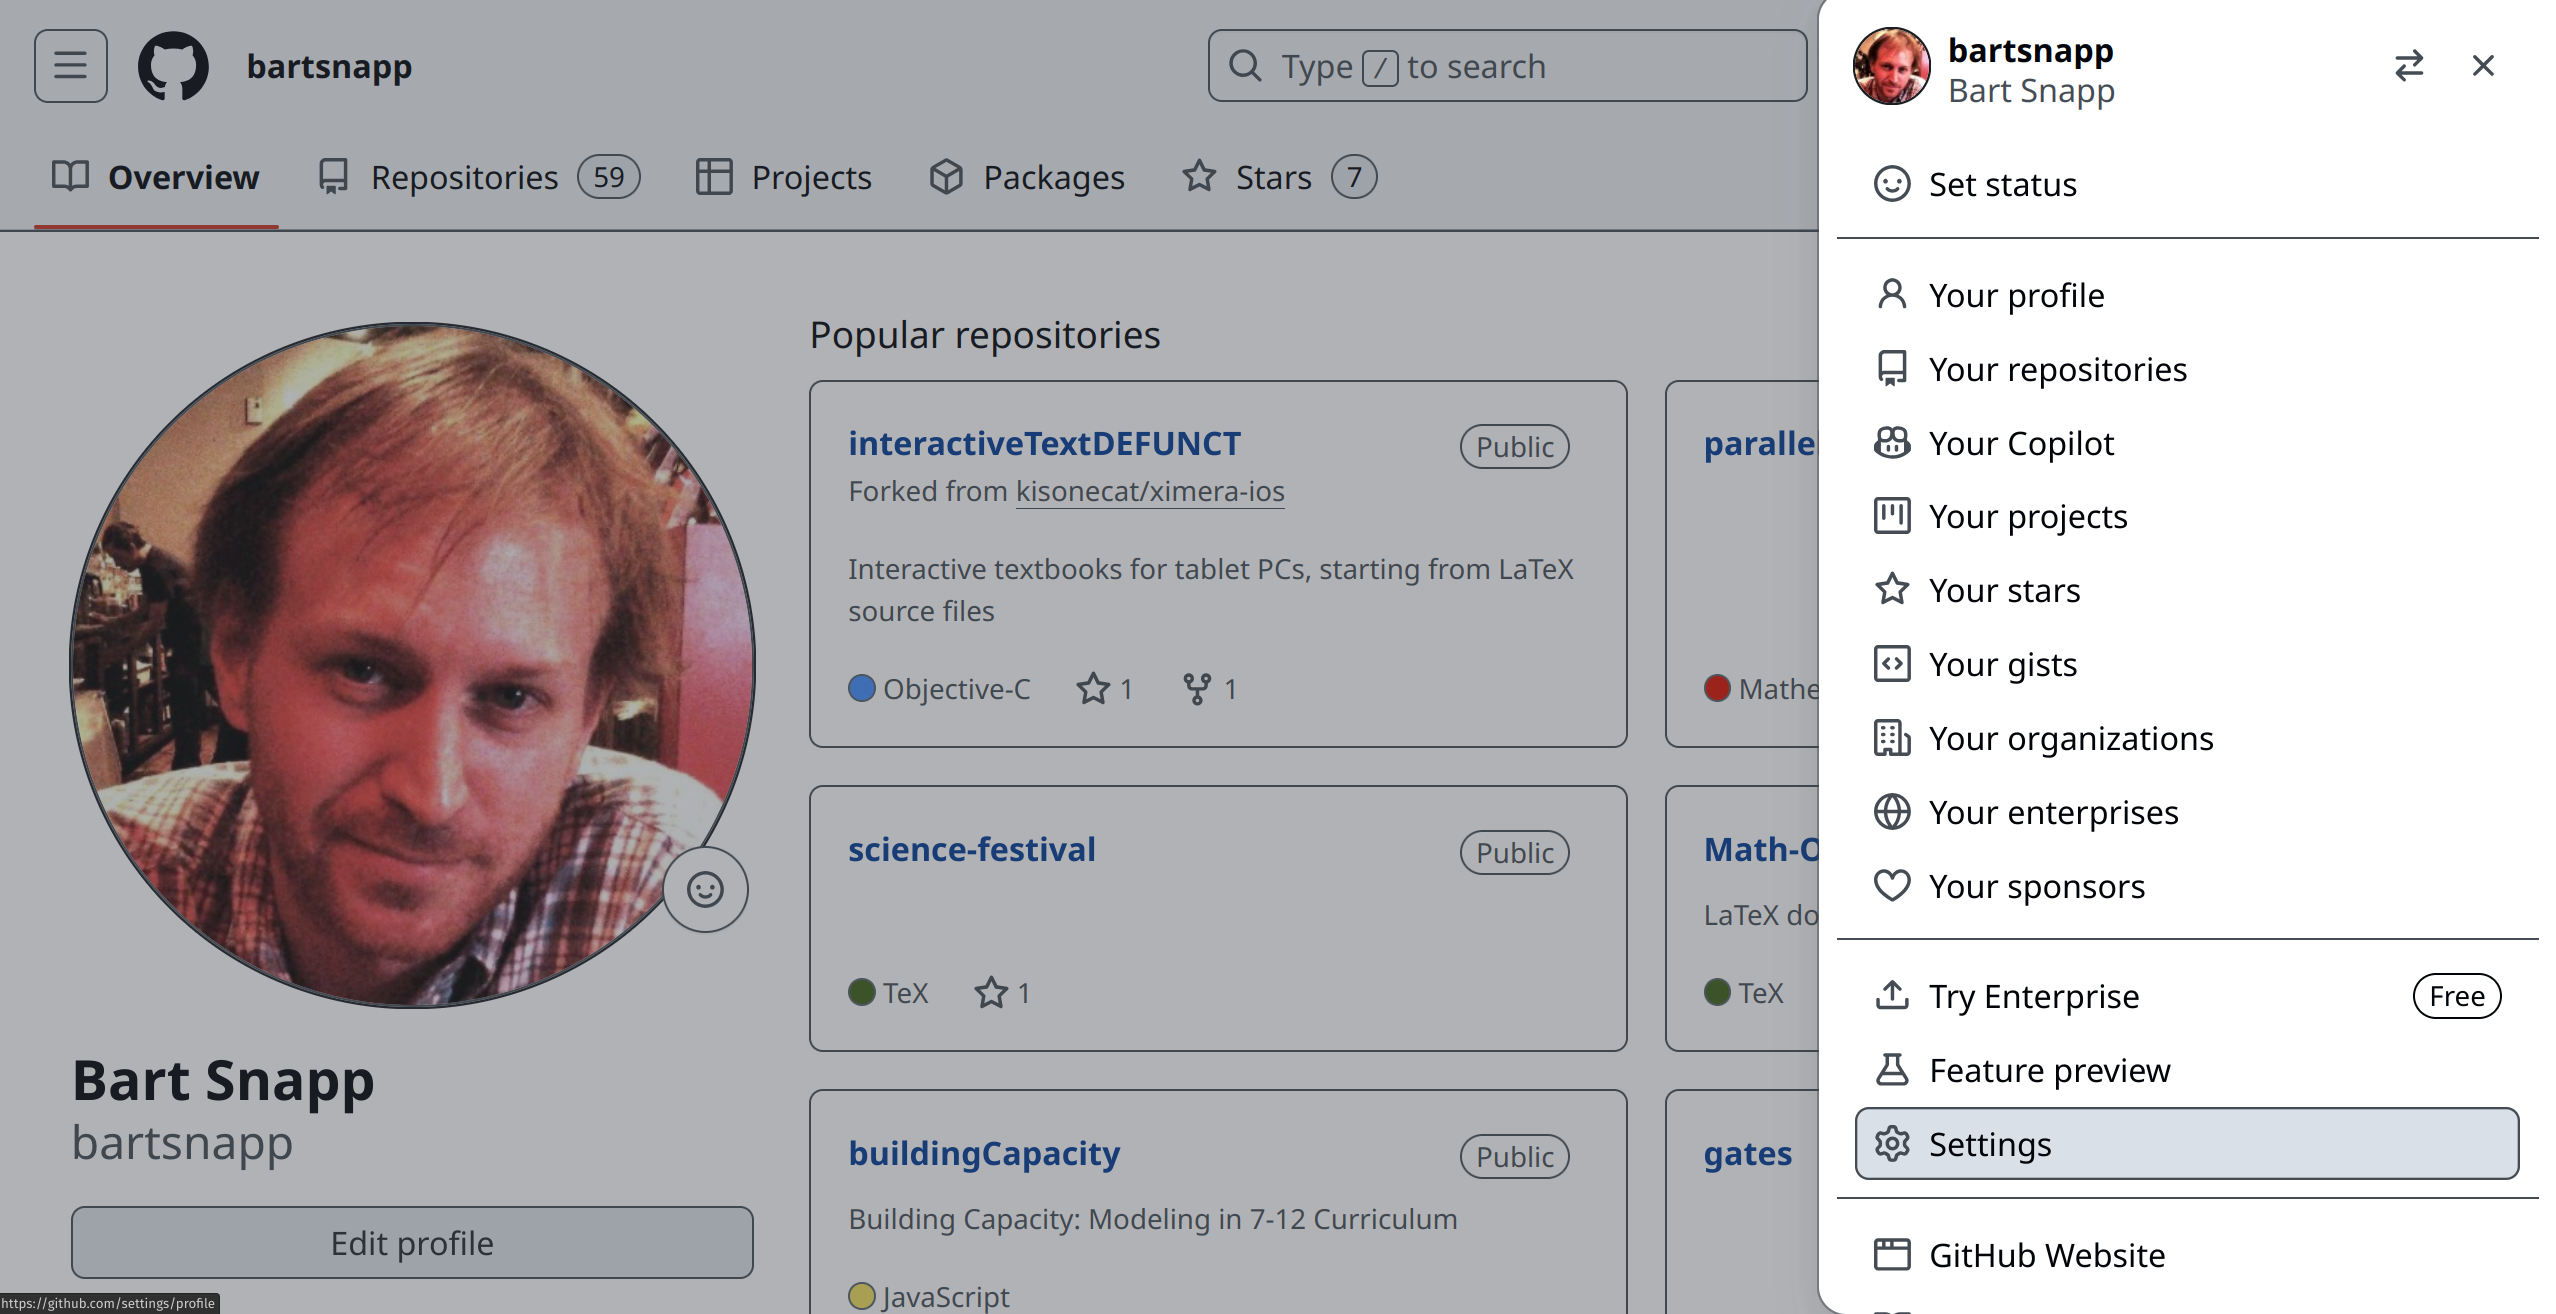
\includegraphics[width=.7\textwidth]{deploySettings.png}
\end{image}
\pdfOnly{\begin{multicols*}{2}}
        \section{GPG keys and codespace}
        Once you have your \verb!GPG_KEY_ID! and \verb!GPG_KEY!, you are ready
        to go.
        Assuming your repository contains the folder \verb!.devcontainer! from
        either
        \verb!ximeraFirstSteps! or \verb!ximeraNewProject!, you can
        start a codespace from GitHub in your web browser and deploy to a
        public-visible
        Ximera server such as: \url{https://ximera.osu.edu}.
        To do this you will need to do some additional set up. You'll need to
        add
        \textbf{two
            new
            secrets to codespace}. Go to your GitHub page, and select
        ``Settings''
        from the
        menu at the top right.

        \pdfOnly{\end{multicols*}}

\pdfOnly{\newpage}

\begin{image}
    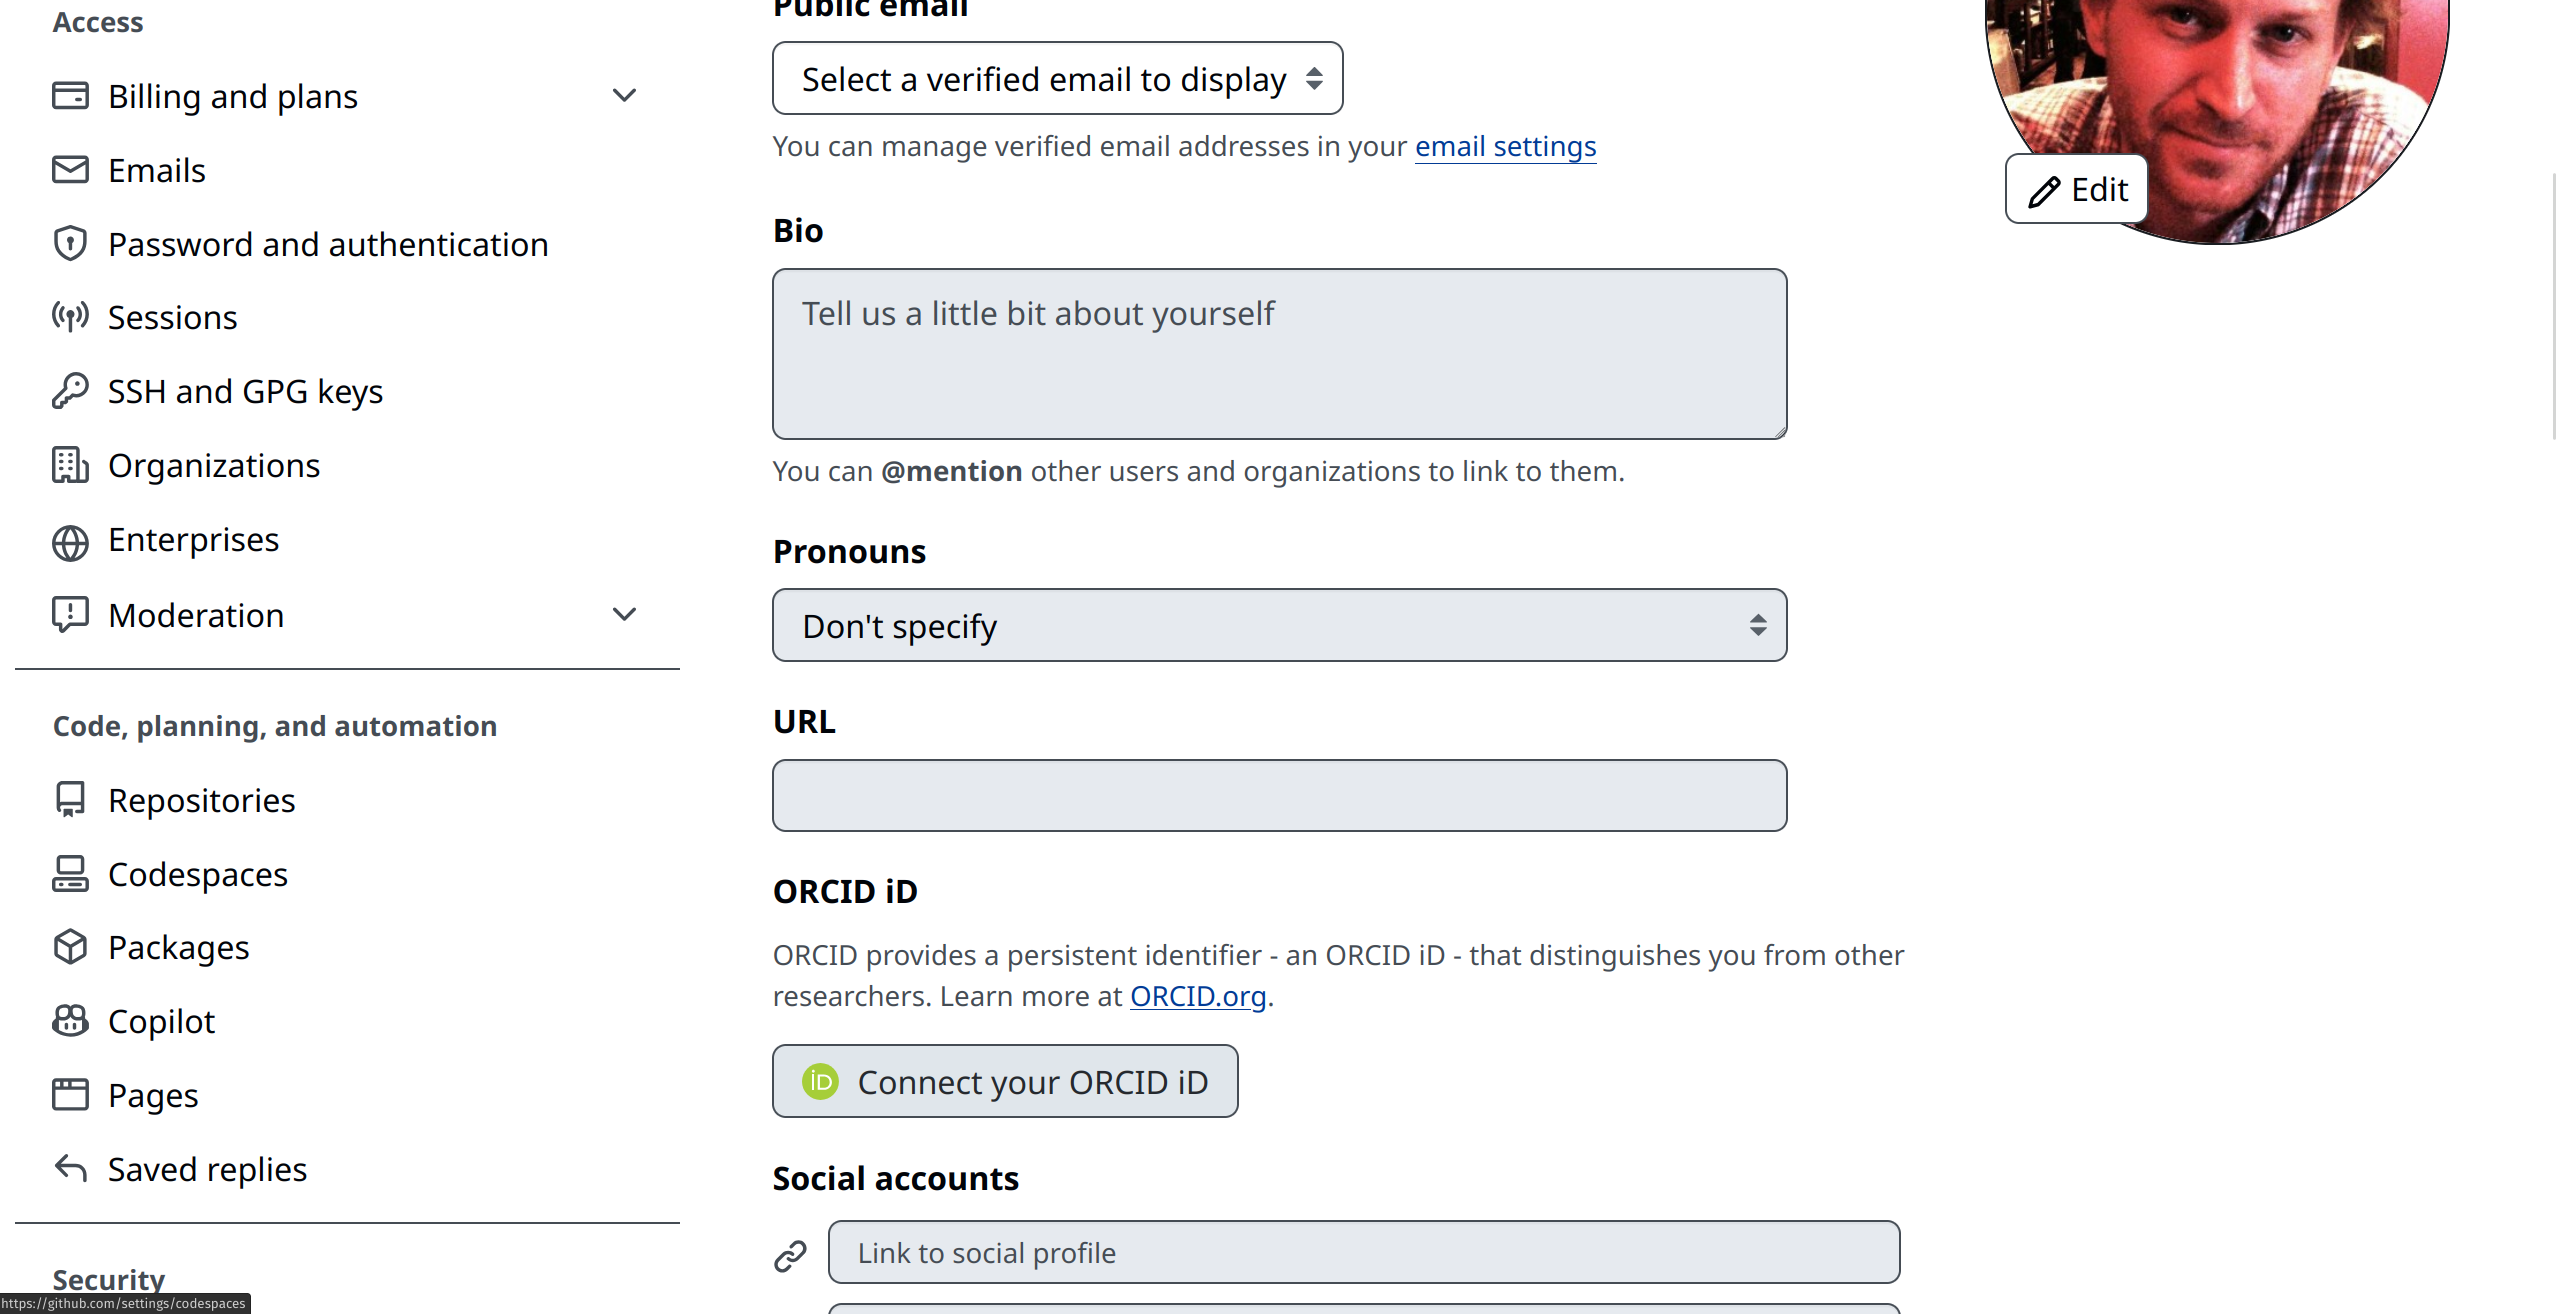
\includegraphics[width=.7\textwidth]{deployClickCodespace.png}
\end{image}

Now look to the left, and scroll down until you see a ``Codespaces'' option.
We see it above.

\newpage

\begin{image}
    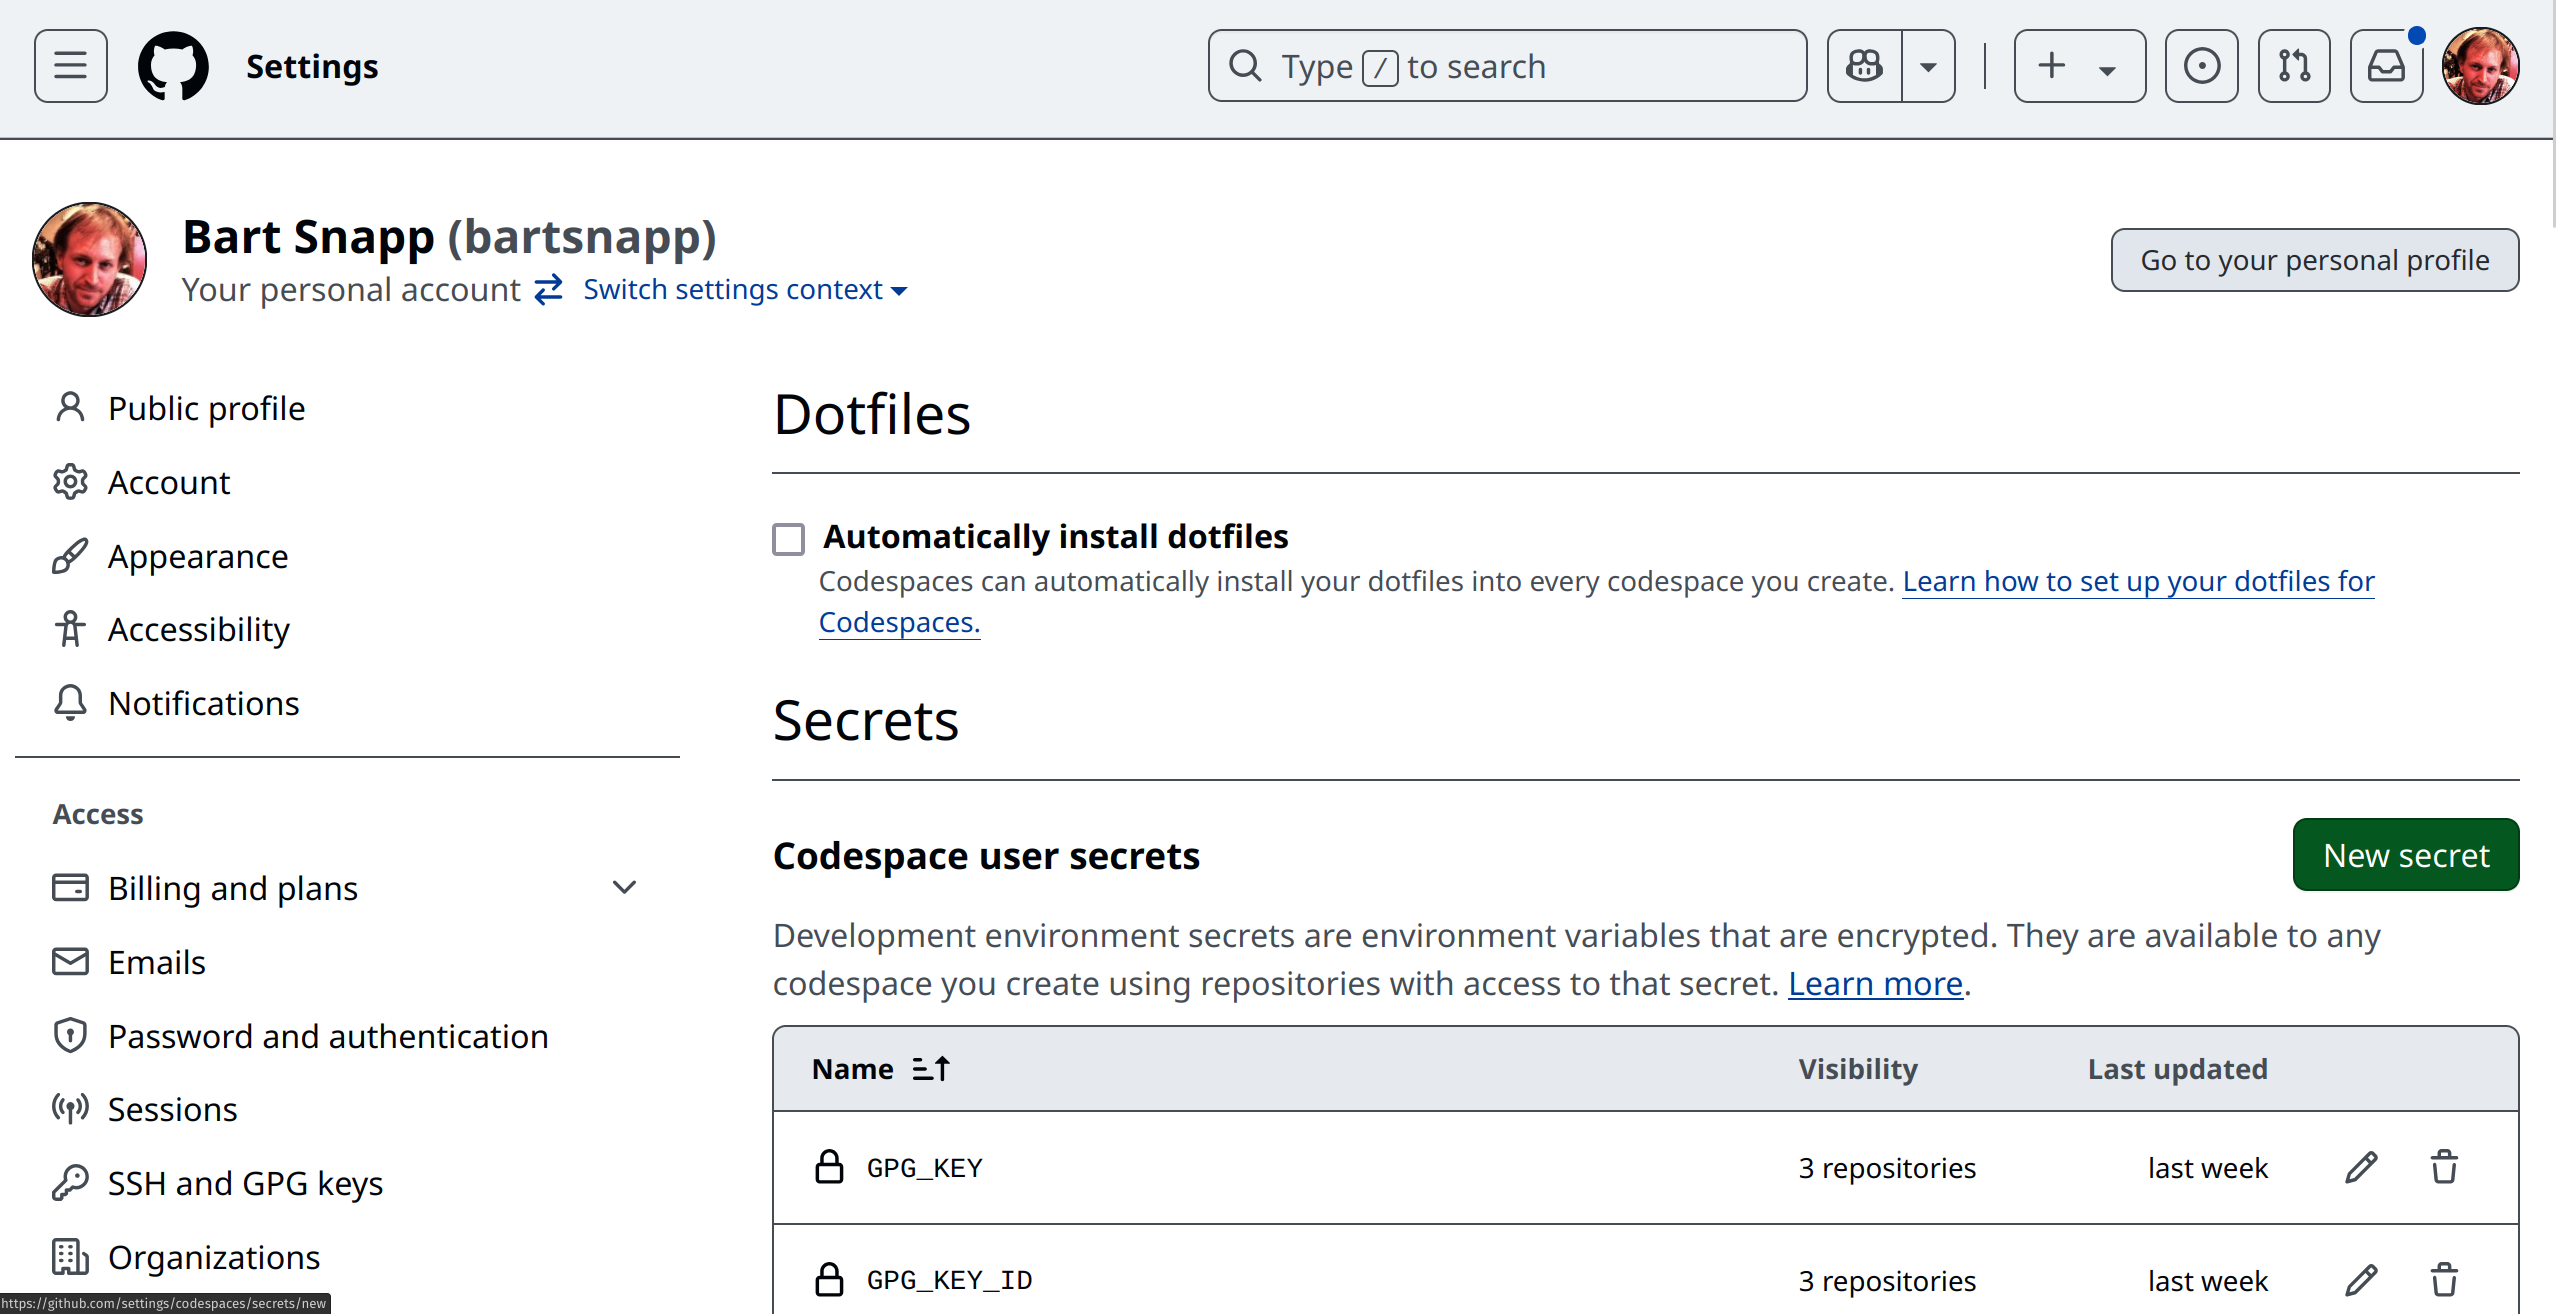
\includegraphics[width=.7\textwidth]{deploySecret.png}
\end{image}

Now click on ``New secret.''

\newpage

\begin{image}
    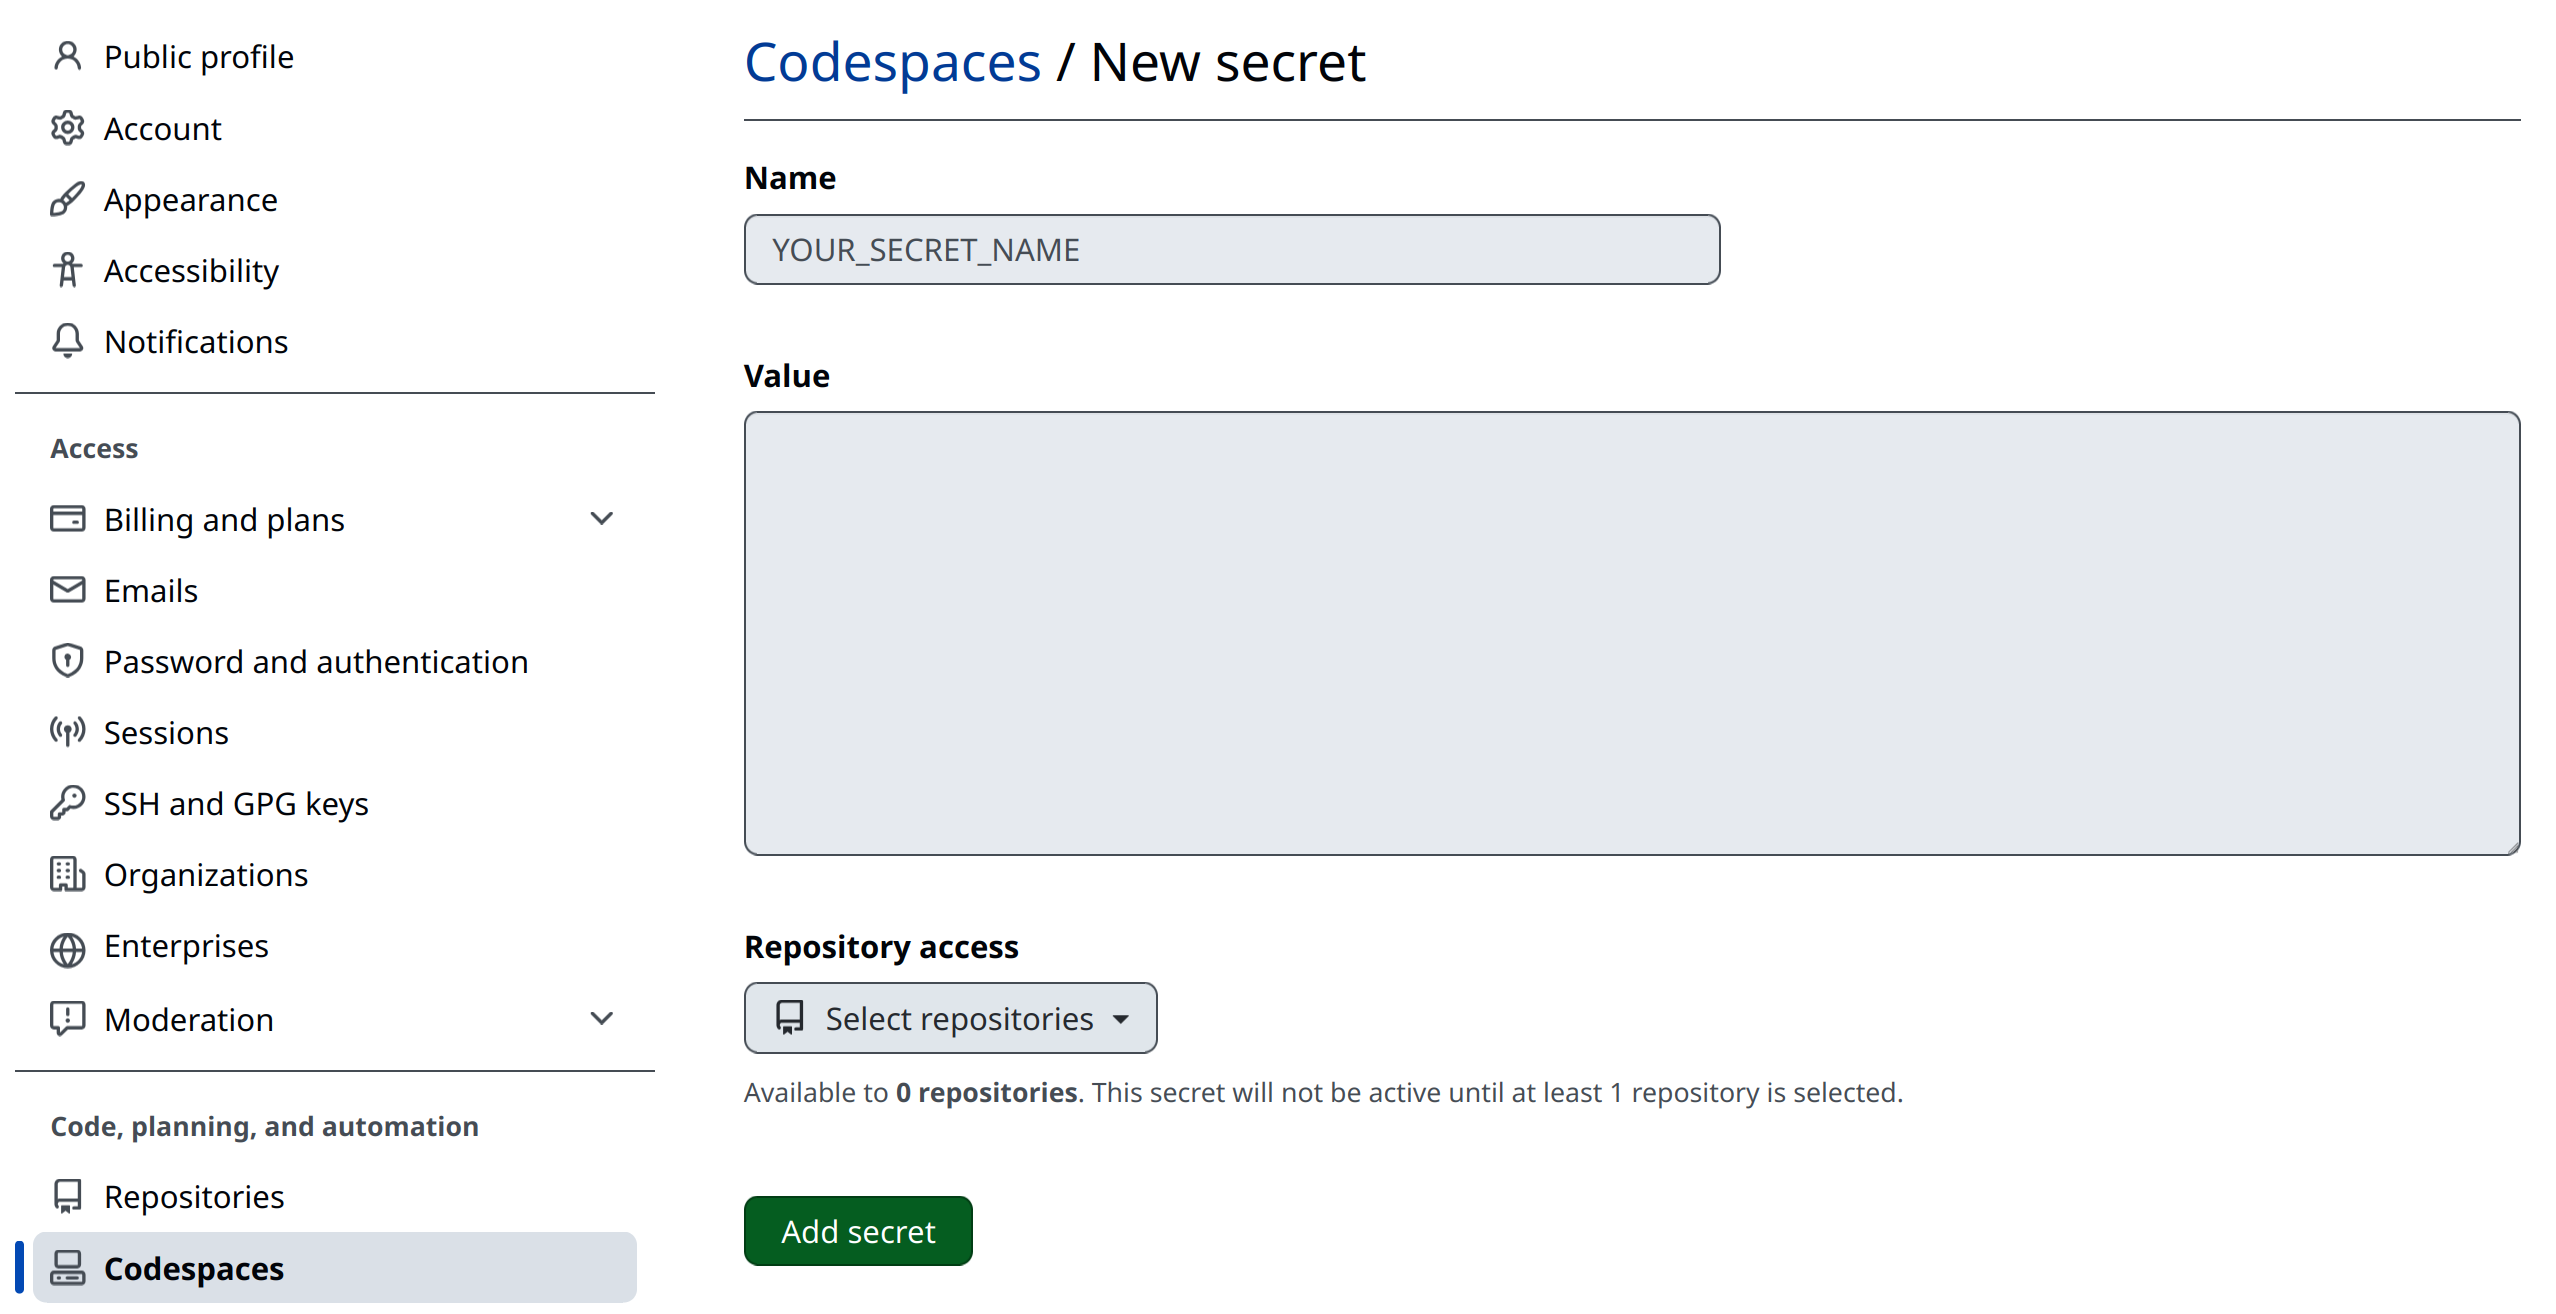
\includegraphics[width=.7\textwidth]{deployID.png}
\end{image}
\pdfOnly{\begin{multicols}{2}}
        Finally, set the name (\verb!YOUR_SECRET_NAME!) of your secrets as:
        \begin{description}
            \item[\texttt{GPG\_KEY\_ID}] with the ``Value'' being the single
                line
                of characters we found before.
                %         \begin{verbatim}
                % 215FC33FAB44D5CCA31A04B2CC78CB561FDC49A8
                % \end{verbatim}
            \item[\texttt{GPG\_KEY}]  with the ``Value'' being the large block
                of
                characters we found before.
                %         something
                %         like:
                %         {\pdfOnly\footnotesize
                %         \begin{verbatim}
                % LS0tLS1CRUdJTiBQR1AgUFJJVkFURSBLRVkgQkxPQ0stLS0tLQoKbEZnRVp2QUFBaFlKS3dZQkJB
                % SGFSdzhCQVFkQUI4UW9zbWR3YmJBcHJHQ1k1N3Q1VmRVVkJGTlpWWEFQTGVkWQpMWnZtQ0tjQUFR
                % QzF4dmlVckwzRWE2bmpJcUZ1WitWL2EzUG55TCtPeDMvTHg3eWxtV2pNNlJUeHRDTkVkVzF0CmVT
                % QkdiM0lnV0dsdFpYSmhJRHh1YjI1bFFHVjRZVzF3YkdVdVkyOXRQb2laQkJNV0NnQkJGaUVFSVYv
                % RFA2dEUKMWN5akdnU3l6SGpMVmgvY1NhZ0ZBbWJ3QUFJQ0d3TUZDUVdqbW9BRkN3a0lCd0lDSWdJ
                % R0ZRb0pDQXNDQkJZQwpBd0VDSGdjQ0Y0QUFDZ2tRekhqTFZoL2NTYWpjaGdFQWhHZkVkYW9xRnZD
                % c21NZExZVmNNSUhkTjl4aXJzZTB1Cjh5WVYweXpGVS9zQSt3Vm9zR3UvYk10b3N2bHphMkRJUkQ3
                % VG9BUE5HeDYwanBlYjJaRm5DQW9LbkYwRVp2QUEKQWhJS0t3WUJCQUdYVlFFRkFRRUhRTitNMW52
                % VG44Um85SFordW50NGJFN1A1dEZ5QnJkbnBmS2pvZ1oyd2R3bApBd0VJQndBQS8xMUhNaFJuTnFL
                % RXpBVC9tN1Y1Mm90NjNjRzNRbFp1R0FFV0tqSmJOZUFJRG9HSWZnUVlGZ29BCkpoWWhCQ0Zmd3or
                % clJOWE1veG9Fc3N4NHkxWWYzRW1vQlFKbThBQUNBaHNNQlFrRm81cUFBQW9KRU14NHkxWWYKM0Vt
                % b2RpTUEvMVBMZFpzc2owdm10VGw1ZEFMUGNMdUpDandNZlgyQWFCS3J1WG0vZjc4UEFQOWM2eHdh
                % YXdSVQpFTks0VCttYU5IbGt6TXVLWjJEYkNwS1Irdk5rdHlWL0FRPT0KPWk3Wk8KLS0tLS1FTkQg
                % UEdQIFBSSVZBVEUgS0VZIEJMT0NLLS0tLS0K
                % \end{verbatim}
                %         }
        \end{description}
        You will also need to select the ``Repository Access'' drop-down menu,
        and give
        the appropriate repositories access to these keys.
        \pdfOnly{\end{multicols}}%% this combined with \twocolumn below is not a mistake

\pdfOnly{\twocolumn} %% this combined with \end{multicols} above is not a mistake

\section{GPG keys on your machine}

This section is for experience GitHub users. To deploy from your machine, you
need a file in
the folder of the repository of
your content that \textbf{is not committed to the repository}. Please reach out
to Ximera developers for help with this step. You will also need to modify
configuration files.

% In essence, you need to put (but not commit) a file like this:
%     {\pdfOnly\footnotesize
%         \begin{verbatim}
% #
% # This file contains a DUMMY GPG key to publish Ximera courses on LOCAL testserver(s).
% #
% #  Use environment variables GPG_KEY_ID and GPG_KEY to overwrite this, or 
% #  change them here with your personal/project GPG key
% #
% #   *** BUT DO NEVER COMMIT THIS FILE WITH REAL KEYS ***
% #
% GPG_KEY_ID=215FC33FAB44D5CCA31A04B2CC78CB561FDC49A8
% GPG_KEY=$(
% cat <<'EOF'
% LS0tLS1CRUdJTiBQR1AgUFJJVkFURSBLRVkgQkxPQ0stLS0tLQoKbEZnRVp2QUFBaFlKS3dZQkJB
% SGFSdzhCQVFkQUI4UW9zbWR3YmJBcHJHQ1k1N3Q1VmRVVkJGTlpWWEFQTGVkWQpMWnZtQ0tjQUFR
% QzF4dmlVckwzRWE2bmpJcUZ1WitWL2EzUG55TCtPeDMvTHg3eWxtV2pNNlJUeHRDTkVkVzF0CmVT
% QkdiM0lnV0dsdFpYSmhJRHh1YjI1bFFHVjRZVzF3YkdVdVkyOXRQb2laQkJNV0NnQkJGaUVFSVYv
% RFA2dEUKMWN5akdnU3l6SGpMVmgvY1NhZ0ZBbWJ3QUFJQ0d3TUZDUVdqbW9BRkN3a0lCd0lDSWdJ
% R0ZRb0pDQXNDQkJZQwpBd0VDSGdjQ0Y0QUFDZ2tRekhqTFZoL2NTYWpjaGdFQWhHZkVkYW9xRnZD
% c21NZExZVmNNSUhkTjl4aXJzZTB1Cjh5WVYweXpGVS9zQSt3Vm9zR3UvYk10b3N2bHphMkRJUkQ3
% VG9BUE5HeDYwanBlYjJaRm5DQW9LbkYwRVp2QUEKQWhJS0t3WUJCQUdYVlFFRkFRRUhRTitNMW52
% VG44Um85SFordW50NGJFN1A1dEZ5QnJkbnBmS2pvZ1oyd2R3bApBd0VJQndBQS8xMUhNaFJuTnFL
% RXpBVC9tN1Y1Mm90NjNjRzNRbFp1R0FFV0tqSmJOZUFJRG9HSWZnUVlGZ29BCkpoWWhCQ0Zmd3or
% clJOWE1veG9Fc3N4NHkxWWYzRW1vQlFKbThBQUNBaHNNQlFrRm81cUFBQW9KRU14NHkxWWYKM0Vt
% b2RpTUEvMVBMZFpzc2owdm10VGw1ZEFMUGNMdUpDandNZlgyQWFCS3J1WG0vZjc4UEFQOWM2eHdh
% YXdSVQpFTks0VCttYU5IbGt6TXVLWjJEYkNwS1Irdk5rdHlWL0FRPT0KPWk3Wk8KLS0tLS1FTkQg
% UEdQIFBSSVZBVEUgS0VZIEJMT0NLLS0tLS0K
% EOF
% )
% \end{verbatim}
%     }
% \begin{enumerate}
%     \item Make sure all source files are committed and pushed to the
%           repository. A quick
%           \begin{verbatim}
% git add -u && git commit -m "this is my change" && git push
% \end{verbatim}
%           may help. Also, you can check your personal GitHub page to ensure
%           files are in
%           the repository.
%     \item Ensure Docker is running.
%     \item Press \textit{Bake} (typically on the bottom taskbar in VS Code).
%     \item Press \textit{Serve} (typically on the bottom taskbar in VS Code).
% \end{enumerate}

% We should discuss this more once the discussion in the repository
% \verb!ximeraFirstSteps! is steady.

\section{Setting the remote Ximera server}

Currently,  \textbf{this is subject to change}, you need to modify:
\begin{verbatim}
xmScripts/config.txt
\end{verbatim}
Around line 20, you will find something like:
\begin{verbatim}
## : "${XIMERA_NAME:=myreponame}"
## : "${XIMERA_URL:=http://localhost:2000/}"
## : "${XIMERA_URL:=https://ximera.osu.edu}"
## : "${XIMERA_URL:=https://set-p-dsb-zomercursus-latest.cloud-ext.icts.kuleuven.be/}"
## : "${XIMERA_URL:=https://set.kuleuven.be/voorkennis/}"
\end{verbatim}
Remove the \verb!##! from the first line, uncommenting it, and set
\verb!myreponame! to be what
you want your content to be called online.
\begin{warning}
    Your name for your content must be \textbf{all lower case} alphanumeric
    English characters. Lower case letters and numbers are fine.
\end{warning}
Next uncomment, remove the \verb!##!, from the line of the server you wish to
deploy to. Save the file. It would probably be best to not commit it to the
repository, though it really doesn't matter. Now, when you press ``SERVE,''
your Ximera content will be deployed online! Please feel free to reach out to
the Ximera developers  for help at this step.

\end{document}
